\documentclass[a4paper,12pt]{article}
%\usepackage{fullpage}
%\usepackage{pdfpages}

\usepackage{geometry}
 \geometry{
 a4paper,
 total={170mm,257mm},
 left=20mm,
 top=20mm,
 }

\usepackage{color}
\usepackage{amsmath,graphicx,makeidx}
\usepackage{lscape}
\usepackage{fancyhdr}
\addtolength{\headheight}{1.5cm} % make more space for the header
\pagestyle{fancyplain} % use fancy for all pages except chapter start
\lhead{
\includegraphics[height=1.7cm]{FOSSEE-logo}} % left logo
\rhead{
\includegraphics[height=3.5cm]{DWSIM-flowsheeting-project-logo}} % right logo
\renewcommand{\headrulewidth}{0pt} % remove rule below header

\title{Removal of Isopentane in Gasoline Manufacturing Plant}
\author{Priyam Nayak \\ Indian Institute of Technology Bombay}
\date{}

\begin{document}

\maketitle

\noindent \textbf{Background \& Description:}
\newline Bypass is an important type of process stream commonly encountered in process industries. It skips one or more stages of the process and goes directly to another downstream stage. A bypass stream can be used to control the composition of a final exit stream from a unit by mixing the bypass stream and the unit exit stream in suitable proportions to obtain the desired final composition.

In a feedstock preparation section of a plant manufacturing natural gasoline, it is important to remove isopentane from butane-free gasoline. In this process, butane-free gasoline consisting of N-pentane and isopentane which are obtained from the bottoms of the debutanizer in the ratio of 4:1 is used as feed. 44.5\% of the butane-free gasoline directly proceeds to the next stage in the natural gasoline plant. Rest of the butane free gasoline is sent to isopentane tower where isopentane is completely removed as top product and N-pentane is obtained from the bottoms. The obtained pure N-pentane is directly sent to natural gasoline plant. Splitter unit of DWSIM is used to bypass a part of the feed stream and compound separator unit is employed for the isopentane tower. 

\vspace{25mm}
\centerline{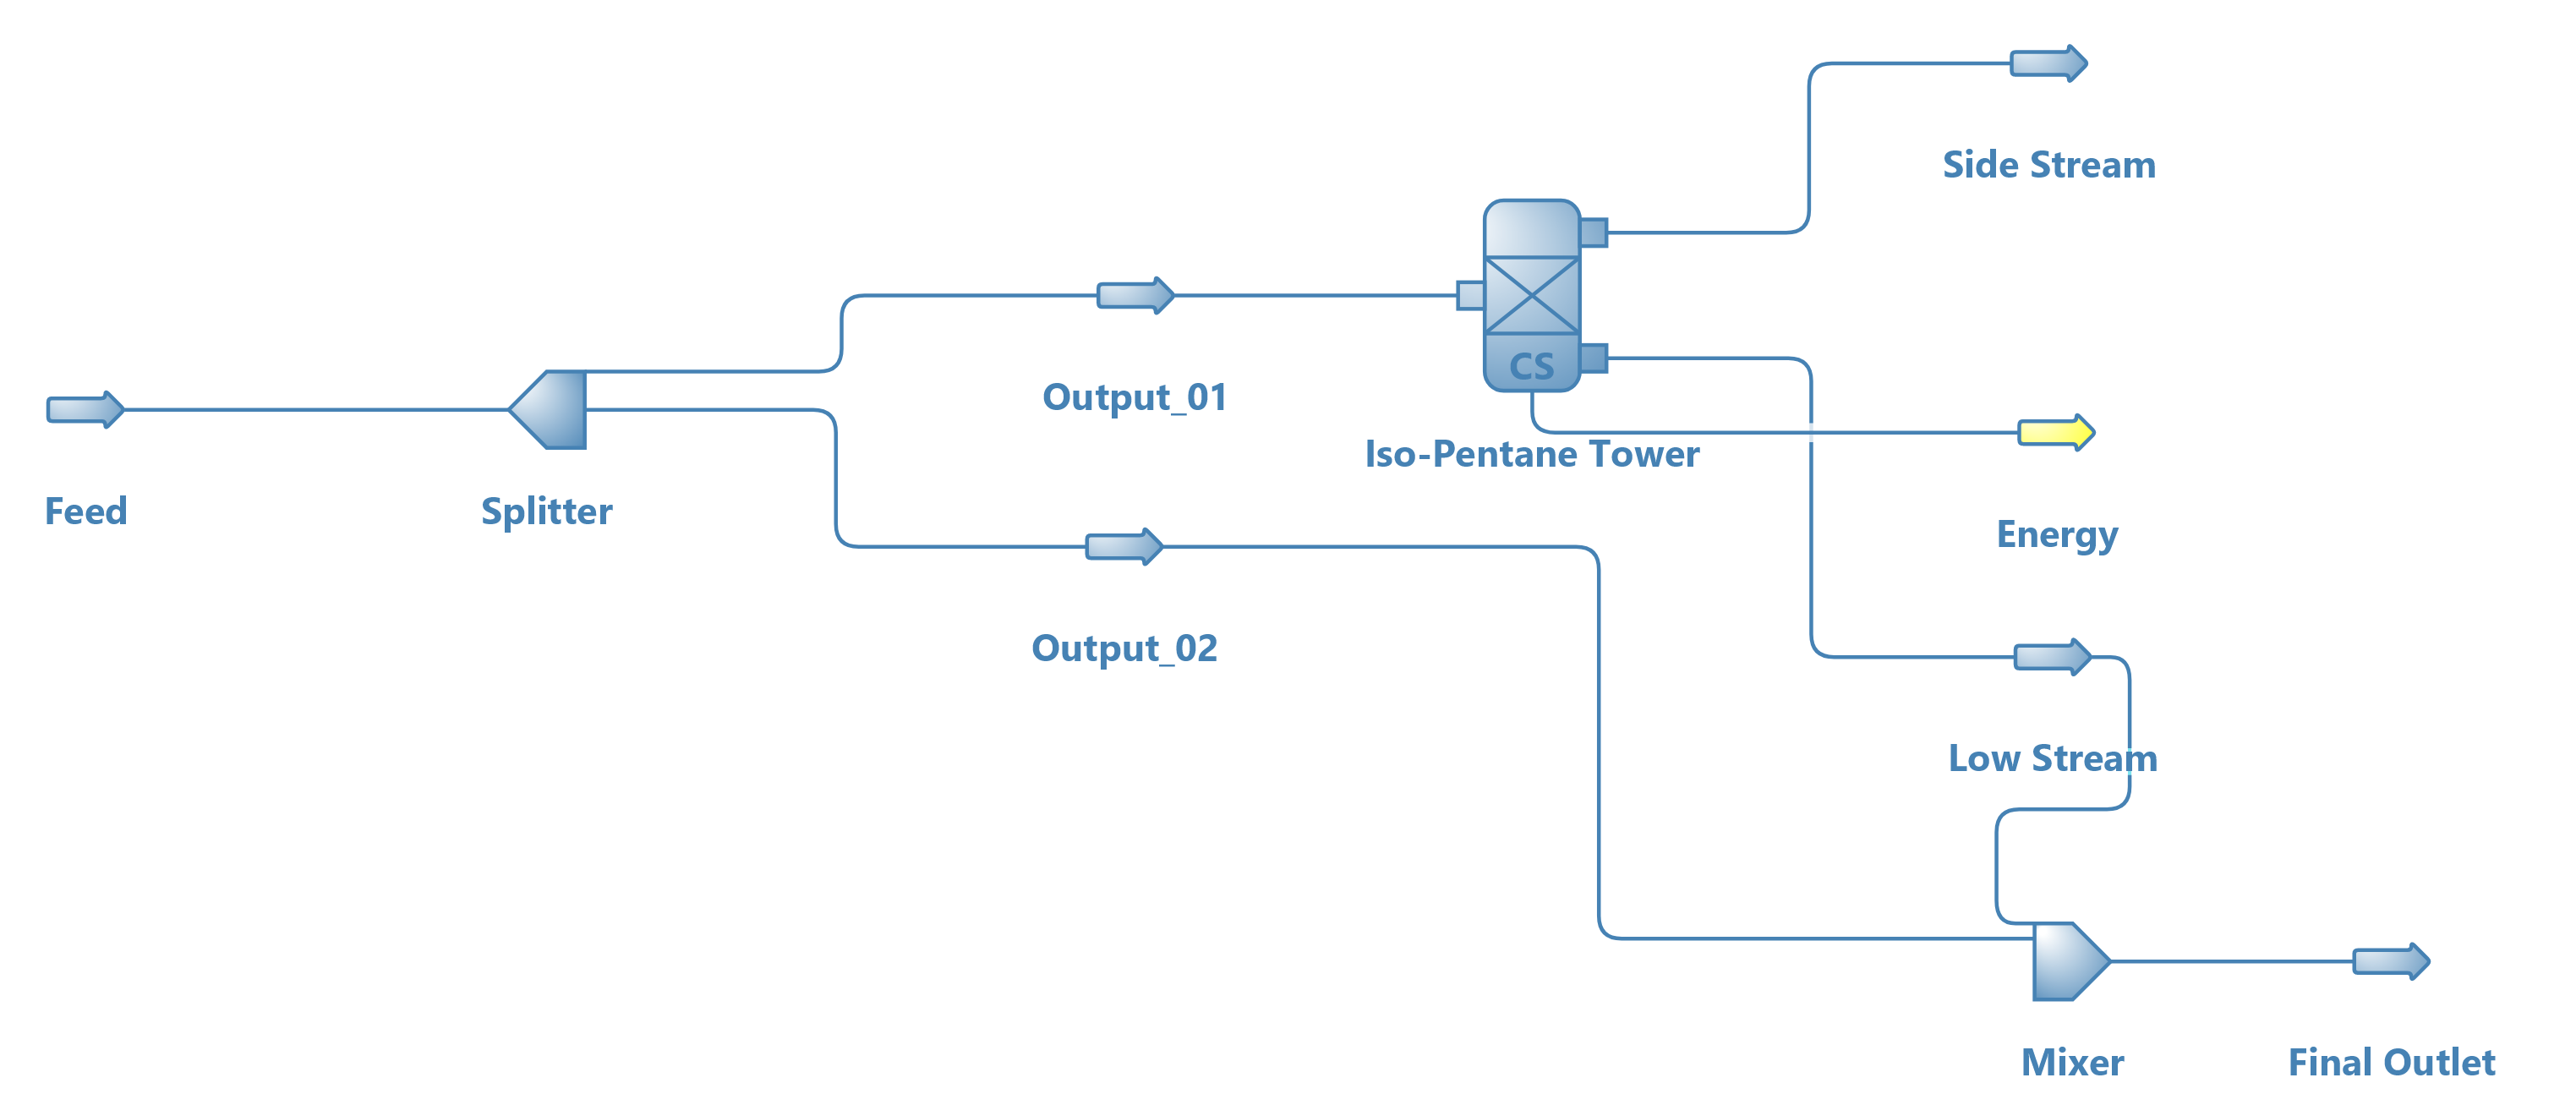
\includegraphics[width=1\linewidth]{Isopent-Rem.png}}


\newpage \noindent \textbf{Results:}
\begin{table}[ht]
\centering
\resizebox{\textwidth}{!}{%
%\resizebox{\columnwidth}{!}{%
%\scalebox{1.2}{%
\begin{tabular}{|l|l|l|l|l|}
\hline
\bf Object                              & Side Stream & Output\_02   & Output\_01 &       \\ \hline
Temperature                         & 298.15      & 298.15       & 298.15     & K     \\ \hline
Pressure                            & 101325      & 101325       & 101325     & Pa    \\ \hline
Mass Flow                           & 11.1        & 44.5         & 55.5       & kg/s  \\ \hline
Molar Flow                          & 153.8462    & 616.7706     & 769.2308   & mol/s \\ \hline
Volumetric Flow                     & 0.01798     & 0.0717       & 0.08942    & m$^3$/s  \\ \hline
Molar Flow (Mixture)  /  N-pentane  & 0           & 493.4165     & 615.3846   & mol/s \\ \hline
Mass Flow (Mixture)  /  N-pentane   & 0           & 35.6         & 44.4       & kg/s  \\ \hline
Molar Flow (Mixture)  /  Isopentane & 153.8462    & 123.3541     & 153.8462   & mol/s \\ \hline
Mass Flow (Mixture)  /  Isopentane  & 11.1        & 8.9          & 11.1       & kg/s  \\ \hline \hline
\bf Object                              & Low Stream  & Final Outlet & Feed       &       \\ \hline
Temperature                         & 298.15      & 297.9408     & 298.15     & K     \\ \hline
Pressure                            & 101325      & 101325       & 101325     & Pa    \\ \hline
Mass Flow                           & 44.4        & 88.9         & 100        & kg/s  \\ \hline
Molar Flow                          & 615.3846    & 1232.155     & 1386.001   & mol/s \\ \hline
Volumetric Flow                     & 0.07144     & 0.14309      & 0.16112    & m$^3$/s  \\ \hline
Molar Flow (Mixture)  /  N-pentane  & 615.3846    & 1108.801     & 1108.801   & mol/s \\ \hline
Mass Flow (Mixture)  /  N-pentane   & 44.4        & 80           & 80         & kg/s  \\ \hline
Molar Flow (Mixture)  /  Isopentane & 0           & 123.3541     & 277.2003   & mol/s \\ \hline
Mass Flow (Mixture)  /  Isopentane  & 0           & 8.9          & 20         & kg/s  \\ \hline
\end{tabular}%
}
\caption{Streamwise Results for Removal of Isopentane in Gasoline Manufacturing Plant}
\end{table}

\end{document}


